\documentclass{beamer}
\usepackage[latin1]{inputenc}
\usepackage{listings}
\usepackage{MnSymbol}
\usepackage{caption}
\usepackage{subcaption}
\usepackage{booktabs}

\DeclareMathAlphabet\mathbb{U}{msb}{m}{n}

\usetheme{Madrid}
\usecolortheme{beaver}


\defbeamertemplate*{title page}{customized}[1][]
{
	\bigskip\bigskip\bigskip\bigskip\bigskip
	\centering{
  \usebeamerfont{title}\inserttitle\par
  \usebeamerfont{subtitle}\usebeamercolor[fg]{subtitle}\insertsubtitle\par
  \bigskip
  \usebeamerfont{author}\insertauthor\par
  \usebeamerfont{institute}\insertinstitute\par
  \usebeamerfont{date}\insertdate\par
  \usebeamercolor[fg]{titlegraphic}\inserttitlegraphic
	\bigskip
	\bigskip
	\usebeamercolor[fg]{normal text}
	\tiny\textbf{Committee}\par
	Murali Sitaraman (Chair)\par
	Brian C. Dean\par
	Jason O. Hallstrom\par
	Roy P. Pargas\par}
\bigskip\bigskip
\includegraphics[width=30px]{NSF_logo}
}


\title[Engineering Specifications and Mathematics]{Engineering Specifications and Mathematics\\for Verified Software}
\author{Hampton Smith}
\institute{Clemson University}
\date{May 16th, 2013}

\lstset{
	escapeinside={[*}{*]},
	basicstyle=\tiny
}

\lstdefinelanguage{Coq}
	{
		morekeywords={Definition,forall,let,Prop,Function,measure,if,then,else,end,match,with,unfold,intro,elim,reflexivity,replace,simpl,intros,split,change,rewrite,omega,assumption,symmetry,apply,auto,Qed,Theorem,functional,induction,in},
		sensitive=true,
		morecomment=[l]{--},
	}

\lstdefinelanguage{resolve}
	{
		morekeywords={restores,of,If,Recursive,Implicit,Powerset,Instance_Of,Theory,Precis,Categorical,introduces,related,Goal,Given,Definition,Facility,is,realized,by,Var,Concept,uses,Defines,Constraints,Initialization,Type,Family,exemplar,initialization,finalization,ensures,Operation,updates,requires,preserves,clears,evaluates,type,Extension,for,end,if,then,replaces,Procedure,convention,correspondence,iff,extended,Enhancement,Realization,represented,alters,in,modeled,constraint,While,changing,maintaining,decreasing,do,Theorem,For,all,implies,where,and,Precis,Subsumption},
		sensitive=true,
		morecomment=[l]{--},
		morecomment=[s]{(*}{*)},
		morestring=[b]",
	}
\lstset{language=resolve}


\begin{document}


\AtBeginSection[]
{
  \begin{frame}<beamer>
    \frametitle{Layout}
    \tableofcontents[currentsection,currentsubsection]
  \end{frame}
}


\begin{frame}
\titlepage
\end{frame}

\section{Introduction}
\begin{frame}{What is verified software?}
	\begin{itemize}
		\item Mathematically prove properties of a program
		\begin{itemize}
			\item No null dereferences
			\item No buffer overflows
			\item No deadlock
			\item Termination
			\item Full behavior
		\end{itemize}
		\item Requires formal semantics
		\item Description of the desired behavior in a formal language
		\item Can be demonstrated by hand or mechanically
	\end{itemize}
\end{frame}


\begin{frame}{How do we verify?}
	\includegraphics[width=\textwidth]{verificationProcess}
\end{frame}


\subsection{Example Systems}
\begin{frame}{Example Systems}
	\begin{columns}
	\begin{column}[l]{5cm}
		Practical Systems
		\begin{itemize}
			\item Existing industrial languages (C, Java)
			\item Limited mathematical language
			\item Focus on verifying narrow properties
			\item Automatic proofs
			\item Accomplishments: Automatically verified linked data structures
			\item Example systems: Jahob, Verifast
		\end{itemize}
	\end{column}
	\begin{column}[r]{5cm}
		Pure Systems
		\begin{itemize}
			\item Research or pure mathematical language
			\item Rich mathematical language
			\item Full verification (up to termination)
			\item Interactive proofs
			\item Accomplishments: Interactively verified C compiler, OS kernel
			\item Example systems: Coq, Issabelle
		\end{itemize}
	\end{column}
	\end{columns}
\end{frame}


\begin{frame}{Jahob Example}
	\lstinputlisting[basicstyle=\tiny,language=Java]{ArrayList1.java}
\end{frame}


\begin{frame}{Coq Example}
	\lstinputlisting[basicstyle=\scriptsize,language=Coq]{DivPred.coq}
	\lstinputlisting[basicstyle=\scriptsize,language=Coq]{DivImpl.coq}
	\lstinputlisting[basicstyle=\scriptsize,language=Coq]{DivTheorem.coq}
\end{frame}


\begin{frame}{Coq Example}
	\lstinputlisting[basicstyle=\scriptsize,language=Coq]{DivProof.coq}
\end{frame}


\begin{frame}{Best of Both Worlds?}
	\begin{itemize}
		\item Practical Systems
		\begin{itemize}
			\item Flexible, integrated specification
			\item Component support
			\item Automatic proofs
		\end{itemize}
		\item Pure Systems
		\begin{itemize}
			\item Modular mathematics and specifications
			\item Protection from certain complications (preferably still with the flexibility to use them)
			\item Rich, extensible mathematical language
		\end{itemize}
	\end{itemize}
\end{frame}

\subsection{Problem Statement}
\begin{frame}{Problem Statement}
	\begin{itemize}
		\item Architecture and implementation of a minimalist rewrite prover to explore those prover capabilities practically necessary to mechanically verify well-engineered, modular components.
		\item Design and implementation of an extensible, flexible supporting mathematical framework for a practical verification system that permits reuse as well as the development of a rich set of models and assertions.
		\item Design and implementation of a well-integrated specification framework that is explicitly designed to work with the mathematical system, supporting verifiability by allowing simple, flexible specifications and supporting scalability by encouraging verified component reuse.
		\item Validation of our central hypothesis via application of the minimalist prover to software constructed using the mathematical and specification framework.
	\end{itemize}
\end{frame}

\begin{frame}{Dissertation Goal}
	In a verification system, an extensible, flexible mathematics and specification subsystem enables better-engineered component specifications and thus more straightforward proof obligations that are easily dispatched by even minimalistic automated provers.  Design, development, and experimentation with such a verification system is the goal of this dissertation.
\end{frame}





\chapter{Minimalist Automated Prover\label{ch:prover}}
%-----------------------------------------------------------------------------
At the core of any mechanical verification system is an automated theorem prover responsible for discharging VCs.  By definition, it is the last word on whether or not a particular technique is yielding more or less easily-proved VCs.  As a result of this, most practical systems have focussed on incorporating the latest and greatest provers into their retinue to piggyback on the breakthroughs at the bleeding edge of proving and artificial intelligence and thus increase provability.

While we are happy to support the latest and greatest suite of provers, we hypothesize that in many cases \emph{flexibility} may trump raw performance with respect to mechanically verifying well-engineered software by encouraging good specification and mathematical engineering that captures the programmer's intuition rather than compromising to work within the framework of a target prover.

In order to experiment with this hypothesis and identify those prover capabilities and performance tunings required to verify well-engineered software, we set out to create a \emph{minimalist automated prover}, starting with only the bare essential capabilities and expanding only when a significant number of VCs appeared that could not be addressed with the prover as it stood.  The result of this effort was RESOLVE's integrated rewrite prover.  As we've refined our design, it has become a platform for prover experimentation within the group and we intend to use it as the yardstick against which to measure our success using our new mathematical system to verify components.


%-----------------------------------------------------------------------------
\section{Original Motivation}
%-----------------------------------------------------------------------------

In practical verification systems to date, specifications are often quite complicated, even for simple operations.  Consider Listing \ref{lst:jmladd} for the JML spec of the \texttt{add()} operation on a \texttt{List} data structure.

\lstinputlisting[language=JML,caption={JML Specification for \texttt{add()}\label{lst:jmladd}}]{JMLAdd.jml}

In this case, the complexity arises from multiple different sources:

\begin{itemize}
	\item The JML specification library seeks to formalize the existing informal specification of the Java Runtime Library, so they are bound by design decisions made agnostic of formal specification.  For example, the original informal specification provides no guidance about how to deal with collections potentially containing more than \texttt{Integer.MAX\_VALUE} elements.
	\item Language complexities like null elements and integer bounds must be taken into account.
	\item Without a correspondence established at the class level between the abstract value of the structure as a whole and its abstract fields, information that would otherwise be redundant must be encoded.  For example, certainly the fact that \texttt{this.contains(o)} follows from \texttt{\\old(this.theCollection.insert(o))}, but no correspondence exists between these two values.
\end{itemize}

Additionally, complexity often arises from other areas as well:

\begin{itemize}
	\item Capturing alias behavior, including the repeated argument problem.
	\item Using separation logic to describe allowable changes in memory while the method call runs.
	\item Poorly designed APIs.
\end{itemize}

The complexity of these specifications necessarily ends up in the VCs that arise from code that operates on these structures.  These complex VCs must then be dispatched by the prover.

The design of RESOLVE, on the other hand, attempts to minimize such complexities.  There are no nulls to reason about.  While integers are bounded, their bounds are asserted in their own component and reasoned about at that level.  A class-level correspondence establishes how the actual fields of the representation map into an abstract value.  RESOLVE minimizes aliasing and marshals reference behavior through a pointer data structure and has a well-defined semantic for repeated arguments.  And while no language can force its users to write good APIs, the constraints and rigor of the language contribute to encapsulated, modular design.  Consider this specification for the comparable \texttt{insert()} operation on the RESOLVE list datastructure:

\begin{lstlisting}[language=RESOLVE]
	ensures P.Prec = #P.Prec and P.Rem = <#New_Entry> o #P.Rem
\end{lstlisting}

While these design decisions were originally made to encourage reuse and simplify \emph{human} reasoning, when we began to be able to generate VCs for various components and algorithms, we noticed they were much more straightforward than those generated by comparable functions.  Consider the VC given in Listing \ref{lst:easyVCEg}.

\lstinputlisting[language=RESOLVE,caption={VC for the Inductive Case of Loop Invariant\label{lst:easyVCEg}}]{StackFlipVC1.asrt}

The VC is easily solvable by expanding the variable S'', then applying a few relatively straightforward transformations on strings.  The presence of these sorts of VCs originally caused us to suspect we could get away with a very simple prover--one that first expanded variables, then substituted equivalent expressions until either the goal matched some given or the expression reduced to \texttt{true}.  To test this hypothesis, we built our first automated prover.


%-----------------------------------------------------------------------------
\section{Version 1 Prover}
%-----------------------------------------------------------------------------

The first prover was extremely straightforward.  As a preprocessing step, it expanded any variables (so for the VC in Listing \ref{lst:easyVCEg}, appearances of both \texttt{S} and \texttt{S''} would be replaced with their full values), then read in theorems from any available theories.  These theorems were applied in alphabetical order by theorem name (in order to ensure consistence between tests) in a depth-first manner, with the search tethered at 6 steps to prevent infinite cycles.

Initially, only equality theorems (i.e., those of the form \texttt{A = B}) were considered, and they were permitted to travel in travel in either direction (i.e., replacing \texttt{A} with \texttt{B} or replacing \texttt{B} with \texttt{A}).

This alone turned out to be sufficient to prove a surprising number of VCs arising from various contexts (for more information, see Chapter \ref{ch:proverEvaluation} for an analysis of the efficacy of these various techniques.)  However, we quickly found VCs like the one given in listing \ref{lst:lessEasyVCEg}.

\lstinputlisting[language=RESOLVE,caption={VC for the Requires Clause of Push\label{lst:lessEasyVCEg}}]{StackFlipVC2.asrt}

The proof for this VC is relatively straightforward: note that \texttt{|S| <= Max\_Depth} and \texttt{S} itself is made up of \texttt{Reverse(S\_Flipped')} and \texttt{S''}.  Since we know that \texttt{|S''| /= 0}, the length of \texttt{Reverse(S\_Flipped')} must be strictly less than \texttt{Max\_Depth}.  Since reversing the string does not affect its length, the length of \texttt{S\_Flipped'} must also be strictly less than \texttt{Max\_Depth}.

However, note that no amount of variable expansion and the application of equality theorems on the consequent will arrive at the solution.  Indeed, even if we expand our process to permit equality theorems to act on the antecedent of the VC, we can't solve it.  What we need is a theorem like:

\begin{lstlisting}
Theorem Non_Empty_Concatenation:
    For all S, T : SStr,
    For all i : Z, 
        |S o T| <= i and |T| /= 0 implies
            |S| < i;
\end{lstlisting}

Since developing the VC's antecedent with a theorem like this is considerably more expensive\footnote{Each conjunct of the antecedent of the theorem must be matched against some given in the antecedent of the VC, and all possible matchings must be considered---making it exponential in the number of VC antecedents, with an order equal to the number of theorem antecedents.}, this was implemented as a preprocessing step, with all available implication theorems applied in three rounds to the antecedent before continuing with the normal proof search using only equality theorems.

This permitted us to dispatch VCs like the one that appeared in Listing \ref{lst:lessEasyVCEg}.  However, at this point we had begun to amass a considerable number of theorems and the time required to successfully search all proofs of length no more than six for a solution was becoming untenable (over a minute to eventually succeed proofs) and we began searching for heuristics to speed up this process.

The first thing we noticed was that \emph{most} VCs required proofs of much shorter length (one, two, or three steps).  So the prover was retrofitted to operate in phases, first searching proofs of length no more than three before trying those of length no more than four and finally trying those no more than six.  This significantly reduced the time to prove many VCs, however still left others taking far too long.

Our second heuristic was to implement a greedy best-first search algorithm by creating a fitness function to determine which theorems were most likely to be helpful on a per-VC basis.  We save discussion of this fitness function for Section \ref{domainSpecific}, where we discuss optimization of the final version of the prover.

	%-----------------------------------------------------------------------------
	\subsection{Implementation}
	%-----------------------------------------------------------------------------

This version of the prover was based on our existing abstract syntax tree data structure.  A recursive loop implemented the main proof search using available equality theorems.  However, a separate, hardcoded pre-processing step performed variable expansions and theory development.


%-----------------------------------------------------------------------------
\section{Version 2 Prover\label{proverV2}}
%-----------------------------------------------------------------------------

As the first prover continued to mature and found its way into our web integrated environment, we continued to experiment with more complex components, including those derived from our burgeoning ideas on specification engineering\cite{smithSpecificationAbstractions} and one born out of our collaboration with the Intelligent River project here at clemson, that required a routine for averaging the integers in a queue datastructure\cite{regula2012case}.  

These new domains yielded VCs that exposed fundamental weaknesses in the first prover and motivated the design and creation of the second prover.  As an example of this sort of VC, consider Listing \ref{lst:longVC}.

\lstinputlisting[language=RESOLVE,caption={VC for the Requires Clause of Advance\label{lst:longVC}}]{longVC.asrt}

This VC expresses a tautology, but requires seventeen steps to prove.  This raised serious concerns that we would not be able to use a simple term-rewrite prover as we had hoped---with hundreds or thousands of theorems in play and combinatorial complexity, it seems impractical to search a proof space that size, even with some guidance about which transformations to prioritize.

Our insight here was that a mathematician, upon seeing this VC, spots a number of simplifications that should ``obviously'' be applied immediately (we subjectively speculate that part of what qualifies a proof step as ``obvious'' is the intuition that there's an extremely low liklihood we will wish to backtrack over that step in the future.)  For example, clearly \texttt{(0 + 1)} adds nothing and should be simplified to \texttt{1}.  Similarly, because of the semantics of \texttt{Left\_Substring}, $\forall S : \text{SStr}, \texttt{Left\_Substring}(S, 0) = \texttt{Empty\_String}$.  And $\forall S : \text{SStr}, \texttt{Empty\_String} o S = S$.

In fact, if we continue to apply such ``obvious'' simplifications until we can quickly reduce the same VC to how it appears in Listing \ref{lst:longVCReduced}.

\lstinputlisting[language=RESOLVE,caption={VC for the Requires Clause of Advance\label{lst:longVCReduced}}]{longVCReduced.asrt}

From here, a four-step proof suffices:

\begin{lstlisting}
|(Right_Substring(S.List, 1))| < 
	|((Reverse((Right_Substring(S.List, 1)))
	 o <Element_At(0, S.List)>))|

|(Right_Substring(S.List, 1))| <                    by (|S o T| = |S| + |T|)
	|Reverse((Right_Substring(S.List, 1)))|
	 + |<Element_At(0, S.List)>|

|(Right_Substring(S.List, 1))| <                    by (|Reverse(S)| = |S|)
	|Right_Substring(S.List, 1)|
	 + |<Element_At(0, S.List)>|

|(Right_Substring(S.List, 1))| <                    by (|<E>| = 1)
	|Right_Substring(S.List, 1)|
	 + 1

true                                                by (i < i + 1)
\end{lstlisting}

We qualified such ``obvious'' steps as those that maintain the tautological property (i.e., could not make a tautologically true VC into one that is not tautologically true) and \emph{strictly reduce} the number of function applications.  We hypothesized that if we could add this to the proof search algorithm as a preprocessing step, we would see improvement on many VCs, however the proof search algorithm of the first prover was such that to do so would require more hard-coding, so we conceived of a new prover, capable of being ``driven'' by an object that described its behavior.  Every action it took would be part of the main proof loop, allowing for the consistent collection of metrics and the easy addition of new kinds of proof steps.

This new prover enabled us to implement the described pre-processing step, which we terming ``Minimization''\footnote{We avoided terms loaded with existing mathematical meaning, such as ``Simplification'', because minimization merely provides a best-effort heuristic for reducing function application count.  Changing the available theorems or even the order of those theorems may affect the outcome of minimization.} using the same machinery as the main proof search, while still allowing us to dictate, e.g., that minimzation should not be backtracked over, while proof steps in the main search might be.

In addition to needing new pre-processing phases, new kinds of proof steps were required for the main proof-space exploration phase.  Motivated by a number of examples that required extensive reasoning about integer bounds---including our queue averaging example and operations on bounded data structures like stacks--we found it was important to be able to strengthen the consequents of a VC by applying implication theorems as well as introduce and instantiate existentially-quantified variables.  The design of the second prover permitted such new kinds of proof rules to be put into place.

\textbf{XXX Need an example! XXX}

	%-----------------------------------------------------------------------------
	\subsection{Implementation}
	%-----------------------------------------------------------------------------

Even had the capabilities of the first prover been sufficient, it suffered from a number of design limitations that we sought to improve in this next iteration.

Our existing AST data-structure was poorly suited for formal reasoning and required constant, defensive deep-copying to ensure that changes made in one area would not propogate to another due to some shared reference.  This was annoying and inefficient.  Exarcerbating this issue, the design of the AST left much to be desired and copying required many scattered, error-prone operations that often failed to copy important data attached to an AST node such as its type.

Additionally, the first prover was insufficiently flexible to permit steps other than equality substitution to be included in the proof-search algorithm without hard coding them.  All pre-processing was hard coded outside the general proof-search algorithm (despite often being sufficient to complete the proof), as was all simplification logic at each step.  In addition to being difficult to understand and upkeep, this made collecting metrics such as run time or proof length difficult to keep, since they could not be applied uniformly to hard-coded steps.

In order to address the shortcomings of the AST, we created a separate data structure to hold expressions that were involved in the proving proces---both those related to the VC itself, and those that were part of theorems.  This structure was immutable and thus permitted references to be passed and subtrees to be shared without fear of the problems usually associated with shared aliases.  Transforming the existing ASTs into this new immutable data-structure also provided a convenient point at which to sanitize and perform defense checks, ensuring that those checks only needed to happen once.

The second prover replaced the hard-coded proof search with a general mechanism that deferred to proving tactic objects that implemented the \emph{Strategy} pattern, permitting a single uniform mechanism by which steps were applied and rolled back, while allowing more flexibility on what exactly constituted a ``step''.  This allowed for consistent metric gathering among a number of other design advantages.  The basic implementation remained a recursive one, with backtracking falling out naturally from unwinding the recursive loop.

%-----------------------------------------------------------------------------
\section{Version 3 Prover}
%-----------------------------------------------------------------------------

While the second prover was much more flexible and brought many new VCs into the realm of provability, we found it did not meet our needs with regard to a number of non-functional attributres unrelated to its strict mathematical power.  This motivated us to develop the third and final version of the prover to address these issues.

	%-----------------------------------------------------------------------------
	\subsection{Issues}
	%-----------------------------------------------------------------------------

		%-----------------------------------------------------------------------------
		\subsubsection{Performance}
		%-----------------------------------------------------------------------------

The second prover eliminated the need to make deep copies at each step by ensuring that VCs were immutable and could thus be safely shared with deeper parts of the recursion.  However, it did this at the cost of eliminating the possibility of making changes to expressions in place---each change had to spawn a completely new structure.  While any unchanged subexpressions could be recycled, this generated a great deal of dynamic memory allocations that slowed down the tight prover loop.

Additionally, while it shared this weakness with the first prover, the second prover's reliance on the old type system, which was plagued with inconsistencies and idiosyncracies, prevented proof states from being hashed efficiently and thus precluded a number of optimizations such as efficiently detecting proof cycles.

		%-----------------------------------------------------------------------------
		\subsubsection{Debugging and Understandability}
		%-----------------------------------------------------------------------------

The capabilities and requirements of our prover are rapidly changing in a research environment and a number of design decisions of the second prover made rapid implementation of new features, or the finding and fixing of bugs very difficult.

Because of the tight recursive loop that applied steps and handled backtracking, adding or modifying cross-cutting concerns such as new metrics, visualizations of proof state, or prover interactions such as timeouts or cancel buttons became very difficult.  This had a corresponding effect on debugging, since introducing tools to examine proof state was correspondingly more difficult, and even setting sane breakpoints became challenging.

Additionally, the object that served to ``direct'' the proof was unweildy and difficult to understand or update.  Many layers of inductive, embedded decisions were represented in a functional way that often required straightforward conceptual decisions (``apply this strategy until it cannot be applied anymore, then move on to this strategy'', ``only apply this strategy if this other one is not applicable'') to be represented in counterintuitive ways.

		%-----------------------------------------------------------------------------
		\subsubsection{Metric Collection}
		%-----------------------------------------------------------------------------

While the second prover was a huge improvement, it still fell short of our metric-collection needs.  Most steps were now governed by the consistent machinery of the main proof loop, but not all.  For example, variable expansion was still the purview of a hard-coded pre-processing step.  Additionally, in order to enable the sorts of complexities we required to be described by the strategy object, what should have been considered entire ``phases'' of the proof were occasionally embedded into a single step that made many different, unrelated modifications to the proof state.

An additional issue was that, with theory development now under the purview of the main prover loop, these steps contributed to proof-length-based metrics.  However, since theory development is purely speculative, in most cases, the vast majority of those steps did not contribute in any useful way to the eventual final proof.  A mechanism was required to trace which steps actually contributed to the eventual result.

		%-----------------------------------------------------------------------------
		\subsubsection{Educational Suitability}
		%-----------------------------------------------------------------------------

While the primary thrust of the RSRG's research is the development of a toolchain to broaden the accessibilty of verified software, another important aspect of our research is the use of formal methods as an educational tool for teaching software engineering.  Because the design of the first two provers had been single-mindedly on mathematical power and cross-cutting concerns were difficult to satisfy under that design, creating visualizations of the proof state, permitting the user to slow down and ``watch'' the automated prover work, or effectively allowing the user to control the course of the proof was very difficult.  Both of the first two versions of the prover had a debug mode in which a window would appear at each step and permit the user to select the next theorem, but it was extremely rudimentary by necessity (see Figure \ref{proverDebugMode}).

\begin{figure}
  \centering
    \includegraphics[width=0.45\textwidth]{proverDebugMode}
  \caption{V1 and V2 Prover Visualization\label{proverDebugMode}}
\end{figure}

		%-----------------------------------------------------------------------------
		\subsubsection{Reliance on Old Type System}
		%-----------------------------------------------------------------------------

The version two prover was still reliant on the old type system to function.  This type system was poorly designed and implemented and would often prevent VCs that were otherwise provable from proving.

	%-----------------------------------------------------------------------------
	\subsection{Design and Implementation}
	%-----------------------------------------------------------------------------

For the third prover, visualization and control of the proof process, along with a design amenable to debugging and the writing of unit tests were made first-class design concerns.  To this end, it eschewed the functional, recursive design of the first two provers in favor of a model/view/controller decomposition.

The third prover maintained the immutable expression data structures of the second version, and replaced the old type system with the new one implemented for Chapter \ref{ch:math}, which also uses immutable structures for the representation of types.

While the expressions are immutable, this version of the prover uses a single, mutable proof state object to hold information about proof state, implementing backtracking via explicit undoing of steps rather than recursive unrolling with copies at each level.  This is significantly more efficient since often a proof step impacts only one small part of the proof state.

Each antecedent in the proof state is wrapped in a object that permits meta-information to be attached about where it came from, this permits the prover to trace backwards on a successful proof and determine exactly which antecedents (and thus exactly which proof steps) contributed to the final result.

Rather than a single strategy object that was built up by composing sub-strategies, the third prover's AI is represented by a \emph{goal stack}, where the top goal is queried each heartbeat and permitted to modify the goal stack or perform a single proof step.  This leads to a much more understandable controller and makes the construction of new goals straightforward.

Much consideration was given to a user interface that would make debugging easy and provide an excellent educational interface.  An image of this interface is provided in Figure \ref{newProverInterface}.

\begin{figure}
  \centering
    \includegraphics[width=0.75\textwidth]{newProverInterface}
  \caption{V3 Prover Interface\label{newProverInterface}}
\end{figure}

The current state of the VC is displayed in (1), while a list of available theorems is displayed in (2).  The textbox at the top of the theorem list allows the user to search theorems based on the symbols it contains.  (3) shows any proof steps taken so far, and clicking on one permits the user to undo it.  Finally, play/stop/pause controls at (4) permit the user to seamlessly transition between interactive and automated proving mode.

When a theorem is selected in interactive mode, any possible applications of that theorem become highlighted in (1) in grey.  Hovering the mouse over a possible application causes it to highlight, and clicking applies the theorem.  If no theorem has been selected from (2), each antecedent of the VC also becomes highlighted and may be selected and applied as an ordinary theorem.

When in automated proving mode, (1) updates periodically with the current state of the proof, allowing the user to visualize the work the prover is doing.  Step functionality is also provided on pause to allow the user to watch the automated prover work step by step.

With fully immutable expressions, a number of optimizations became possible.  Proof state is efficiently hashed using a polynomial hash that can be rapidly updated as expressions are added or removed.  This permits us to rapidly detect proof cycles and prune those parts of the tree from the search.  Memoization was used when comparing types to ensure that once we establish a particular type relationship (which can be quite costly under the new analysis), we never calculate it again.  Finally, both the singleton and flyweight patterns were used along with object pools to minimize dynamic object creation.

Finally, for the collection of metrics, the final version of the prover outputs significantly more data in a significantly more readable form than either earlier version.  These proof files include all productive steps of the proof, with a snapshot of the VC at that time, as well as metrics about the proving process, such as length and elapsed time.

\textbf{XXX Insert a figure of this output when it's working XXX}

	%-----------------------------------------------------------------------------
	\subsection{Domain-Specific Optimizations\label{domainSpecific}}
	%-----------------------------------------------------------------------------

An important hypothesis of this research is that a cutting-edge automated prover should not be required to prove the sorts of VCs that arise from well-engineered code.  To this end a significant thrust of our experimentation with the prover was developing heuristics that assist it in dispatching not general mathematical statements, but rather the sorts of obligations that arise from code.

Each heuristic technique is presented at a high level here, and data on its effectiveness is presented in Chapter \ref{ch:proverEvaluation}.

 		%-----------------------------------------------------------------------------
		\subsubsection{Intelligent Antecedent Development}
		%-----------------------------------------------------------------------------

Antecedent development refers to the process of establishing new known facts based on existing ones.  For example, given \texttt{A ---> B} as a VC and a theorem stating \texttt{A ---> C}, we may develop the VC's antecedent into \texttt{A and C ---> B}.  Because such developments always hold true and may often be efficiently searched, it is generally useful to spend some time expanding our list of known facts before embarking on our proof search.  In some sense, this increases the size of the ``target'' we're trying to hit--since transforming the consequent into a match for \emph{any single} antecedent allows us to establish the VC.

However, given the comparatively-large number of knowns at any step of a program (almost always more than is strictly neccessary to establish the VC), combined with the large number of available theorems and their frequently closed nature, blindly adding antecedents results in a combinatorial explosion of required space that yields a low number of useful facts compared to irrelevant ones.  We therefore use a number of heuristics to attempt to improve this situation.

\paragraph{Qualify and Ignore Useless Transformations.}  As part of our goal for RESOLVE to remain scalable, we seek to insulate the end users---whether the programmer or the mathematician---from the details of the prover.  To this end we have routinely rejected designs and methodologies that require the theory developer to ``tag'' theorems or otherwise provide hints to the prover inside a theory or program, a technique that is frequently employed by other mathematical reasoning systems (see, e.g., \cite{kaufmannACL2}).

First, note that while we often use language such as ``applying a theorem'', there is not a one-to-one correspondence between a theorem, which is a general statements of mathematical truth, and the ways that it can be applied.  For example, a theorem that states \texttt{A = B} could be applied to reduce the expression \texttt{A = B} to \texttt{true}, or to replace an \texttt{A} with a \texttt{B}, or in the other direction to replace a \texttt{B} with an \texttt{A}.  We term these individual ways of applying a theorem \emph{transformations}.

Despite our lack of human-provided hints about theorems, it is often possible to qualify different kinds of resulting transformations and thus treat them differently based on their unique usefulness in a given situation.  We use this technique to limit useless antecedent development by ``spotting'' identity functions and refusing to apply them to complexify a known fact.  For example, consider this theorem from \texttt{String\_Theory}:

\begin{lstlisting}
Theorem Concatenate_Empty_String_Identity_Right:
	For all S : SStr, S o Empty_String = S;
\end{lstlisting}

Certainly, to apply this theorem from left to right would often be useful, but to apply it in the other direction adds little to the coverage of our antecedent.  The antecedent development stage therefore ignores such identity-maintaining transformations when they increase the number of function applications.

\paragraph{Develop Only About Relevant Terms.}  It is very often the case that a VC contains many irrelevant antecedents providing information that is not useful to the final proof.  While in general it is not possibile to sort relevant from irrelevant without first arriving at a proof, we recall that we expect all VCs to be straightforward and thus apply a simple heuristic: a new antecedent should only be considered useful if it tells us something about a term that appears in the consequent\footnote{We take note of any equalities such as \texttt{A = B}, where \texttt{A} and \texttt{B} are terms, to permit developments about terms that are equivalent to terms that appear in the consequent.}.

While in a general proof system, this would limit our useful developments, since proofs might be quite deep, based on our hypothesis that reasoning should be straightforward we expect that any required information should already be available roughly in the vocabulary of the consequent.

\paragraph{Maximize Diversity.}  Any transformation that may be applied to develop the antecedent has a dual that could be instead applied to the consequent.  We've therefore tried to explore which kinds of steps are most advantageous during the antecedent development phase and which are better left for the consequent exploration phase.  Intuitively, we note that the antecedent development phase, which occurs once as a preprocessing step and requires no back-tracking, is an ideal place to apply more computationally expensive steps; by contrast, the consequent exploration phase, which does not accumulate related facts and is therefore not subject to a combinatorial explosion of space, is an ideal place to explore many small variations.  We therefore hypothesized that antecedent-development time would be best spent establishing varied facts that put antecedents in new terms.  To qualify this, we added the requirement that each antecedent introduced must both eliminate some term and introduce one.

Take, for example, this partial VC:

\begin{lstlisting}
|S| > 0
  --->
S /= Empty_String
\end{lstlisting}

We would permit the development \texttt{|S| /= 0}, since it eliminates the greater-than symbol and introduces the not-equal symbol, but not \texttt{|S| > 0 + 1}, since, while it introduces two symbols, it does not eliminate any.

\paragraph{Maintain Simplicity.}  We discussed our minimization algorithm in Section \ref{proverV2}.  After each round of antecedent development, we minimize the resultant antecedents.  This provides two advantages: first, it supports the diversity maximization from above by exposing antecedents that essentially establish the same fact in the same terms (which are then removed as redundant); second, it increases the liklihood of transforming the consequent into an antecedent during the proof exploration phase, since both antecedents and consequent orbit the same ``normal form''.

 		%-----------------------------------------------------------------------------
		\subsubsection{Intelligent Consequent Exploration\label{consequentExploration}}
		%-----------------------------------------------------------------------------

Consequent exploration refers to the final phase of the proof search during which the consequent is repeatedly transformed using available theorems until it reduces to \texttt{true} or the search times out.

However, given the large number of available theorems and their frequently closed nature, the consequent space to be explored is extremely large, suffering from a combinatorial explosion of time.  It therefore becomes important to search this space in a reasonable manner, since in general an exhaustive search will be computationally infeasible.

\paragraph{Minimize Complications.}  Before beginning consequent exploration in earnest, we apply the minimization algorithm described in Section \ref{proverV2}.  This eliminates many complications that to a human user would consitute ``obvious'' steps.

\paragraph{Qualify and Ignore Useless Transformations.}  As during antecedent development, we identify transformations that simply introduce identity functions and ignore them during our proof search.

\paragraph{Detect Cycles.}  While the VC state itself is mutable, all components of the state (the expressions and their types) are immutable, which lends itself to efficient calculation of expression hashes.  Using a polynomial hash, the overall hash of the VC state can be updated in constant time each time an expression is added, removed, or modified.  In this way, we can efficiently detect cycles and thus not bother to inductively explore beyond them.

This ability also supports our desire to divorce theory creation from reasoning about the prover in the following way: mathematical systems like ACL2\cite{kaufmannACL2} and Issabelle\cite{wenzelIsar} require theorems to be annotated with the direction in which they should be applied in order to prevent cycles that arise from the same theorem being applied repeatedly backward and forward.  Our prover is able to detect such a situation and avoid it.

\paragraph{Tether Search.}  The main consequent exploration algorithm is a depth-first search.  While cycle-detection eliminates one class of infinite, unproductive path, others exist.  For example: the prover might repeatedly add one to both sides of an equation.  Consistent with our hypothesis that VCs should be straightforward to prove, we tether the search to a short length, after which no further exploration will be applied.  While this depth is parameterizable, we've found that the default of four is generally sufficient.

\paragraph{Step Intelligently.}  Rather than step blindly, we apply a greedy best-first algorithm in our search.  In order to quantify what we mean by ``best'', we must establish a useful fitness function for each transformation.  Empirically, we found that re-calculating fitness at each step was far too costly in terms of time, but we are able to find a sensible ordering of available theorems on a per-VC basis.

We identified three criteria on which to determine the fitness of a transformation: 1) what affect does applying the transformation have on the unique symbols present?  Does it introduce new unique symbols?  Does it eliminate existing ones? 2) what affect does applying the transformation have on the number of function applications? 3) how many symbols does the transformation share with the VC?

After experimentation, the third criteria was not useful, since a transformation attempting to match symbols not contained in the VC can never be applied, and thus any such symbols that might be \emph{produced} by the transformation, must be newly unique, which is subsumed by the second criteria.

By deprioritizing transformations that will introduce new symbols, we prevent the prover from ``entering new territory'' before it's finished exploring all the ways it can transform the current symbols.  Similarly, by deprioritizing transformations that increase the number of function applications, we encourage proof states toward simplicity and parsimony that are easier to explore.  In a \emph{general} proof system, we might assert that these tactics were just as likely to lead us \emph{away} from a correct proof as to bring us closer, but in the specific domain of verifying well-engineered software, we hypothesize that the programmer is not taking leaps of logic and thus the reasoning should be simple.

\section{Mathematical Flexibility}

\lstset{
	basicstyle=\footnotesize
}


\subsection{Design}
\begin{frame}{Mathematical Flexibility: Motivation}
	\begin{itemize}
		\item Mathematical system is the language of specification
		\item It is the source of an increase in effort for verified software
		\item Therefore, it needs to be familiar and its results reusable
		\item Pure systems contain many useful features that practical systems do not take advantage of
	\end{itemize}
\end{frame}

\begin{frame}{Mathematical Flexibility: Contributions}
	\begin{itemize}
		\item We demonstrate how a number of features from pure systems (higher-order definitions, first-class types, etc.) can be utilized to ease the verification task in a practical system
		\item We provide a mathematical foundation for several pre-existing RESOLVE features
		\item We introduce novel tools for static reasoning in the presence of dependent types
		\item For full details, see Chapter 5
	\end{itemize}
\end{frame}



\begin{frame}{Tools for Static Reasoning}
	\begin{itemize}
		\item First-class types permit undecidable type relationships
		\item Nonetheless, static typing is a useful tool
		\item \emph{Type theorems} are a novel compromise introduced by this research
	\end{itemize}
	\vspace{2em}
	\lstinputlisting[language=resolve,caption=]{examples/typeTheorem1.mt}
\end{frame}

\begin{frame}{Tools for Static Reasoning}
	\begin{figure}
		\centering
		\includegraphics[width=.6\textwidth]{../typeGraph.png}
	\end{figure}
\end{frame}


\subsection{Evaluation}
\begin{frame}{Sorting a Queue}
	\lstinputlisting[basicstyle=\tiny,language=resolve,caption=]{../mathEval/examples/Sorting_Capability.en}
\end{frame}

\begin{frame}{Sorting a Queue}
	\lstinputlisting[basicstyle=\tiny,language=resolve,caption=]{../mathEval/examples/String_Theory1.mt}
\end{frame}

\begin{frame}{Sorting a Queue}
	\lstinputlisting[basicstyle=\tiny,language=resolve,caption=]{examples/String_Theory2.mt}
\end{frame}

\begin{frame}{Sorting a Queue}
	\lstinputlisting[basicstyle=\tiny,language=resolve,caption=]{../mathEval/examples/totalpreorderingvc.asrt}
\end{frame}

\begin{frame}{Sorting a Queue}
	\lstinputlisting[basicstyle=\scriptsize,language=resolve,caption=]{examples/preorderingTheorem.mt}
\end{frame}

\begin{frame}{Error Analysis and Reporting}
~
\end{frame}


\begin{frame}{Array Realization of a Stack}
	\lstinputlisting[basicstyle=\tiny,language=resolve,caption=]{../mathEval/examples/Array_Realiz1.rb}
\end{frame}

\begin{frame}{Array Realization of a Stack}
	\lstinputlisting[basicstyle=\tiny,language=resolve,caption=]{../mathEval/examples/Binary_Iterator_Theory1.mt}
\end{frame}

\begin{frame}{Error Analysis and Reporting}
~
\end{frame}


\begin{frame}{Classroom Experiment}
	\begin{itemize}
		\item Mathematical development assignment given to a graduate-level programming languages class for extra-credit
		\item Example demonstrating first-class types and type theorems
		\item No formal training
		\item Assignment asked increasingly difficult questions: last three required analysis and adaptation\\
		\begin{enumerate}
			\item Asserts that \texttt{Without\_Last\_Zero(10)~=~1}.  This may require an extra step to establish proper symbols.
			\item Asserts that for any multiple of ten, \texttt{t,~Next\_Even(t)~mod~10~=~2}.  This may require some additional steps to establish proper symbols and relationships.
			\item Asserts that for all multiples of ten, \texttt{t}, and integers, \texttt{i}, \texttt{Without\_Last\_Zero(t~*~i)~=~i}.  This may require some additional steps.
		\end{enumerate}
	\end{itemize}
\end{frame}

\begin{frame}{Classroom Experiment}
	\begin{itemize}
		\item 7/9 students participated
		\item All but one student successfully completed questions 10 and 11 correctly
		\item Two of the seven completed 12 correctly
	\end{itemize}
\end{frame}





\section{Conclusions and Future Directions}
\begin{frame}{Conclusion}
	\begin{itemize}
		\item Systems need not be limited to the features of a pure or a practical system. Our hybrid system incorporates features of practical verification systems (static checking, efficient implementation, polymorphism) with pure mathematical systems (dependent types, higher-order logic, mathematical reusability.)
		\item Novel mechanism for static reasoning can be used to bridge the gap between undecidable, but flexible type systems and constrained, hierarchical systems.
		\item It can be demonstrated empirically that using such a language, a programmer is capable of creating components about which reasoning is sufficiently easy that VCs can be dispatched by a minimalist prover.
		\item This includes a verified generic sorting algorithm---a first.
		\item A variety of useful heuristics exist to help a minimalist prover expose programmer intuition.
	\end{itemize}
\end{frame}

\begin{frame}{Future Directions}
	\begin{itemize}
		\item Better transformation fitness functions
		\item Other prover styles
		\item Evaluate usability of new features
		\item Increase type-system intuitiveness
		\item Prover scalability
	\end{itemize}
\end{frame}


\begin{frame}{Questions?}
~
\end{frame}

\begin{frame}{Type Universe}
	\centering
	\includegraphics[width=.5\textwidth]{../universe}
\end{frame}

\begin{frame}{Specification Style}
	\lstinputlisting[language=resolve,caption=]{examples/specificationStyle.co}
\end{frame}

\begin{frame}{Implicit}
	\begin{figure}
	\centering
	\begin{tabular}{lrrrr}
		\toprule
			& Time (ms)	& $\sigma$& Steps & Search \\
		\midrule
		VC 0\_1	& 1520		& 141	& 5 	& 0     \\
		VC 0\_2	& 3118		& 295	& 7 	& 0     \\
		VC 0\_3	& 2741		& 222	& 8 	& 0     \\
		VC 0\_4	& 2174		& 170	& 9 	& 2     \\
		VC 1\_1	& 366		& 83	& 10	& 0     \\
		\bottomrule
	\end{tabular}
	\caption{Recursive \texttt{Flipping\_Capability} results\label{fig:flippingResults}}
\end{figure}
\end{frame}

\begin{frame}{Explicit}
	\begin{figure}
	\centering
	\begin{tabular}{lrrrr}
		\toprule
			& Time (ms)	& $\sigma$& Steps & Search \\
		\midrule
		VC 0\_1	& 2199		& 160	& 5 	& 0     \\
		VC 0\_2	& 1468		& 182	& 6 	& 0     \\
		VC 0\_3	& 2149		& 253	& 8 	& 0     \\
		VC 0\_4	& 1589		& 225	& 8 	& 3     \\
		VC 1\_1	& 845		& 139	& 10	& 0     \\
		\bottomrule
	\end{tabular}
	\caption{Recursive \texttt{Flipping\_Capability} results, based on an explicitly-specified queue\label{fig:explicitFlippingResults}}
\end{figure}
\end{frame}

\begin{frame}{Comparison}
	\begin{itemize}
		\item Explicit 1669 ms longer
		\item Saved two proof steps
		\item Cost one search step
	\end{itemize}
\end{frame}

\end{document}
